\documentclass[10pt]{beamer}
\usepackage{graphicx} % Required for inserting images
\usepackage{amssymb}
\usepackage{amsmath}
\usepackage{amsthm}
\usepackage{hyperref}

%\usepackage{listings}
%\usepackage{fancyhdr}
%\usepackage{xcolor}
%\usepackage{geometry}
%\usepackage{ragged2e}
%\usepackage{subcaption}
%\usepackage{multirow}
%\usepackage{tabularx}
%\usepackage{indentfirst}
%\usepackage{lscape}
%\usepackage{titlesec}
%\usepackage[nottoc,numbib]{tocbibind}
%\usepackage[usenames, dvipsnames]{xcolor}
%\usepackage{tikz} \usetikzlibrary{calc}
%%\usepackage[boxed, linesnumbered]{algorithm2e}
%\usepackage{algpseudocode}
%\usepackage{algorithm}

\usetheme{Madrid}
\usecolortheme{seahorse}

\beamertemplatenavigationsymbolsempty


\title[PCCA]{\textbf{Advanced Vector Extensions for modular arithmetic}}
\date{20 May 2025}
\author[D.ASSIRE, M.BONBOIRE]
{Damien ASSIRE \and Marie BONBOIRE}

\AtBeginSection[]
{
  \begin{frame}
    \frametitle{Table of Contents}
    \tableofcontents[currentsection]
  \end{frame}
}


\begin{document}

\begin{frame}[plain]
	\begin{center} 
		
\includegraphics[scale=0.1]{su.png}
    \end{center}

    \titlepage
    
    \vfill
    \begin{flushleft}
        {\small
            \textbf{Supervisor:} Mr. Vincent NEIGER\footnote{\url{https://vincent.neiger.science/}} (LIP6 - PolSys)\\
        }
    \end{flushleft}
\end{frame}

\begin{frame}
    \frametitle{Table of Contents}
    \tableofcontents
\end{frame}

\section{Preface}
\begin{frame}
    \frametitle{Introduction}

    \textbf{Environment}
    \begin{itemize}
        \item C Language,
        \item Fast Library for Number Theory (FLINT) library v. 20.0.0,
        \item Ring $\mathbb{Z}/n\mathbb{Z}, n < 2^{64}$.
    \end{itemize}

    \medskip
    \textbf{State-of-the-art}
    \begin{itemize}
        \item Intel HEXL library\cite{boemer2021intelhexlacceleratinghomomorphic}
        \item Mathemagix library\cite{vanderhoeven2014modularsimdarithmeticmathemagix}
    \end{itemize}

    \medskip
    \textbf{Machines description}
    \begin{center}
        \scalebox{0.5}{
        \begin{tikzpicture}[very thick, black]

            %coordinates
            \coordinate (O) at (0,0); % Origin
            \coordinate (F) at (9.25,0); %End
            \coordinate (P1) at (1,0); %ppti
            \coordinate (P2) at (4.75,0); %groebner
            \coordinate (P3) at (8.25,0); %mariz+argiope

            %proc
            \draw[<-,thick,color=black] ($(P1)+(0,0.2)$) -- ($(P1)+(0,1.5)$) node [above=0pt,align=center,black] 
            {Intel® xeon® Gold 6248 Processor \\ (Cascade Lake, AVX512) \\ 2.5 GHz};
            \draw[<-,thick,color=black] ($(P2)+(0,0.2)$) -- ($(P2)+(0,0.7)$) node [above=0pt,align=center,black] 
            {Intel® xeon® Gold 6354 \\ (Ice Lake, AVX512) \\ 3.0 GHz};
            \draw[<-,thick,color=black] ($(P3)+(0,0.2)$) -- ($(P3)+(0,1.5)$) node [above=0pt,align=center,black] 
            {AMD Ryzen 7 PRO 7840U \\ (Zen 4, AVX512) \\ 3.3 GHz};
            \draw[<-,thick,color=gray] ($(P3)-(0,0.6)$) -- ($(P3)-(0,1.5)$) node [below=0pt,align=center,gray] 
            {Intel(R) Core(TM) Ultra 5 125H \\ (Meteor Lake) \\ 4.5 GHz};

            %main arrow
            \draw[->] (O) -- (F);

            %ticks
            \foreach \x in {1,4.75,8.25}
            \draw(\x cm,3pt) -- (\x cm,-3pt);
            %labels
            \foreach \i \j in {1/2019,4.75/2021,8.25/2023}{
            	\draw (\i,0) node[below=3pt] {\j} ;
            }
        \end{tikzpicture}
        }
    \end{center}
\end{frame}

\begin{frame}
    \frametitle{Introduction}

    \textbf{Vectorization}
    
    Goal: Use SIMD instructions to improve performance for some modular arthmetic operations

    \begin{itemize}
        \item Use SIMD from AVX families (AVX2 and AVX512)
            \begin{itemize}
                \item Used with Intel intrinsics
                \item Tested compiler auto-vectorization vs manual vectorization
            \end{itemize}
        \item uops.info tables give timings for SIMD for different processors
    \end{itemize}
    
    \bigskip
    \textbf{Timings measurement}

    Compared timings from different versions using profiling function
    \begin{itemize}
        \item[$\rightarrow$] Test those versions with diffrent input sizes
    \end{itemize}
\end{frame}

\section{Multiplication of 64-bit integers}
\subsection{Long multiplication}
\begin{frame}
    \frametitle{Long multiplication}
    Let $x,y$ be two integers of at most 64 bits, $0 < k \leq 32$, we write:
    \begin{align*}
        x &= x_{hi} \cdot 2^k + x_{lo}, \\
        y &= y_{hi} \cdot 2^k + y_{lo}.
    \end{align*}

    \pause
    \begin{mybox}
        The product $xy$ by the \textit{long multiplication} is given by
        $$xy = r_{lo} + (r_{mi} \ll k) + (r_{hi} \ll 2k)$$
        where:
        \begin{align*}
            r_{lo} &= x_{lo} \cdot y_{lo}, \\
            r_{mi} &= x_{lo} \cdot y_{hi} + x_{hi} \cdot y_{lo}, \\
            r_{hi} &= x_{hi} \cdot y_{hi}. 
        \end{align*}
    \end{mybox}
\end{frame}

\subsection{Retrieve the high and the low part of the result}
\begin{frame}
    \frametitle{Retrieve high and low part of the result}
    \begin{mybox}
        The product $xy$ is represented as:
        \begin{align*}
            (xy)_{lo} &= (r_{hi} \ll 2\cdot k) + (r_{mi} \ll k) + r_{lo}, \\
            (xy)_{hi} &= (r_{hi} \gg (64 - (2\cdot k))) + (r_{mi} \gg (64 - k)) + carry_{lo},
        \end{align*}
        such that $xy = (xy)_{hi}\cdot 2^{64} + (xy)_{lo}$.
    \end{mybox}

    \pause
    \begin{itemize}
        \item \code{mullo(a,b)}: multiply the $x$-bit integers in $a$ and $b$, producing intermediate $2x$-bit integers, 
        and store the low $x$ bits of the intermediate integers.
        \item \code{mulhi(a,b)}: multiply the $x$-bit integers in $a$ and $b$, producing intermediate $2x$-bit integers, 
        and store the high $x$ bits of the intermediate integers.
    \end{itemize}

    \pause
    \medskip
    \textbf{FLINT} $\longrightarrow$ \code{umul\_ppmm}

    \pause
    \medskip
    \textbf{AVX512} $\longrightarrow$ \code{\_mm512\_mullo\_epi64}

    \begin{table}[h!]
        \centering
        \scalebox{0.7}{
        \begin{tabularx}{0.9\textwidth} { 
            | >{\centering\arraybackslash}X 
            | >{\centering\arraybackslash}X
            | >{\centering\arraybackslash}X 
            | >{\centering\arraybackslash}X | }
            \hline
            \rowcolor{myGray} 
            Processor & Cascade Lake & IceLake & Zen 4 \\
            \hline
            \cellcolor{myGray} Throughput & 1.5 & 3.0 & 1.0 \\
            \hline
        \end{tabularx}
        }
        %\caption{Throughputs of the instruction \texttt{vpmullq zmm, zmm, zmm}.}
    \end{table}
\end{frame}

\subsection{Modular multiplication with a precomputation step}
\begin{frame}
    \frametitle{Modular multiplication with a precomputation step}

    \begin{mybox}
        Let $B$ be the maximum bit size of a word ($B\in \{32, 64\}$). \\
        Given $n$ and $w \in \mathbb{Z}/n\mathbb{Z}$, one can compute a \textit{scaled approximation} 
        of $\frac{w}{n}$: $$ w_{pre} = \biggl\lfloor\dfrac{w\cdot 2^{B}}{n} \biggr\rfloor.$$
    \end{mybox}

    \pause
    \bigskip
    For a vector $b = (b_1,\dots, b_N) \in (\mathbb{Z}/n\mathbb{Z})^N$, we compute 
    $$(w\cdot b_i \mod n) \text{ for each } i\in \{1, \dots, N\}$$

    using \textbf{Shoup algorithm}\cite{Bos_Stam_2021}:
    \medskip
    \begin{enumerate}
        \item compute $p_{hi}, p_{lo}$ such that $w_{pre} \cdot b_i = p_{hi}\cdot 2^B + p_{lo}$, \hfill (1 \code{mulhi})
        \item $c \gets w\cdot b_i - p_{hi}\cdot n$, \hfill (2 \code{mullo})
        \item if $c \geq n$, return $c-n$, else return $c$ \\
            $\Longleftrightarrow \min(c-n, c)$.
    \end{enumerate}
\end{frame}

\section{Classic arithmetic operations on vectors}
\subsection{Addition of two vectors}
\begin{frame}
    \frametitle{Vector addition with a 60-bit modulus (1)}

    \begin{table}[h!]
        \centering
        
        % Proc 1: ppti
        \begin{tabular}{|r|*{3}{c c|}}
            \hline
            \rowcolor{myGray} 
            \multicolumn{7}{|c|}{\textsc{Cascade Lake}} \\
            \hline
            \rowcolor{myGray}
            Ver.\textbackslash N & 510 & & 2010 & & 32768 & \\
            \hline
            \cellcolor{myGray} Seq. & 1.57e-07 & 1.0x & 7.17e-07 & 1.0x & 1.35e-05 & 1.0x \\
            \hline
            \cellcolor{myGray} AVX2 & 1.25e-07 & 3.7x & 6.77e-07 & 2.7x & 1.31e-05 & 2.1x \\
            \hline
            \cellcolor{myGray} AVX512 & 9.34e-08 & 5.8x & 6.73e-07 & 3.1x & 1.27e-05 & 2.4x \\
            \hline
            \cellcolor{myGray} FLINT & 1.50e-07 & 4.3x & 8.10e-07 & 2.9x & 1.56e-05 & 2.3x \\
            \hline
        \end{tabular}
    
        % Proc 2: groebner
        \begin{tabular}{|r|*{3}{c c|}}
            \hline
            \rowcolor{myGray} 
            \multicolumn{7}{|c|}{\textsc{Ice Lake}} \\
            \hline
            \rowcolor{myGray}
            Ver.\textbackslash N & 510 & & 2010 & & 32768 & \\
            \hline
            \cellcolor{myGray} Seq. & 7.55e-08 & 1.0x & 3.34e-07 & 1.0x & 1.14e-05 & 1.0x \\
            \hline
            \cellcolor{myGray} AVX2 & 7.74e-08 & 4.1x & 2.93e-07 & 4.5x & 9.59e-06 & 2.5x \\
            \hline
            \cellcolor{myGray} AVX512 & 1.80e-07 & 4.0x & 4.90e-07 & 4.1x & 1.36e-05 & 1.8x \\
            \hline
            \cellcolor{myGray} FLINT & 1.50e-07 & 5.5x & 3.75e-07 & 5.6x & 1.80e-05 & 2.6x \\
            \hline
        \end{tabular}
    
        % Proc 3: argiope
        \begin{tabular}{|r|*{3}{c c|}}
            \hline
            \rowcolor{myGray}
            \multicolumn{7}{|c|}{\textsc{Zen 4}} \\
            \hline
            \rowcolor{myGray}
            Ver.\textbackslash N & 510 & & 2010 & & 32768 & \\
            \hline
            \cellcolor{myGray} Seq. & 7.17e-08 & 1.0x & 3.66e-07 & 1.0x & 6.16e-06 & 1.0x \\
            \hline
            \cellcolor{myGray} AVX2 & 5.27e-08 & 4.7x & 3.48e-07 & 3.4x & 6.55e-06 & 2.7x \\
            \hline
            \cellcolor{myGray} AVX512 & 5.91e-08 & 4.3x & 3.58e-07 & 3.2x & 5.97e-06 & 3.0x \\
            \hline
            \cellcolor{myGray} FLINT & 5.55e-08 & 4.9x & 3.43e-07 & 3.1x & 6.61e-06 & 3.0x \\
            \hline
        \end{tabular}
        %\caption{Timings in seconds and ratios of the modular sum with a 60-bit modulus.}
    \end{table}
\end{frame}

\begin{frame}
    \frametitle{Vector addition with a 60-bit modulus (2)}

    \begin{figure}[h!]
        \begin{center}
            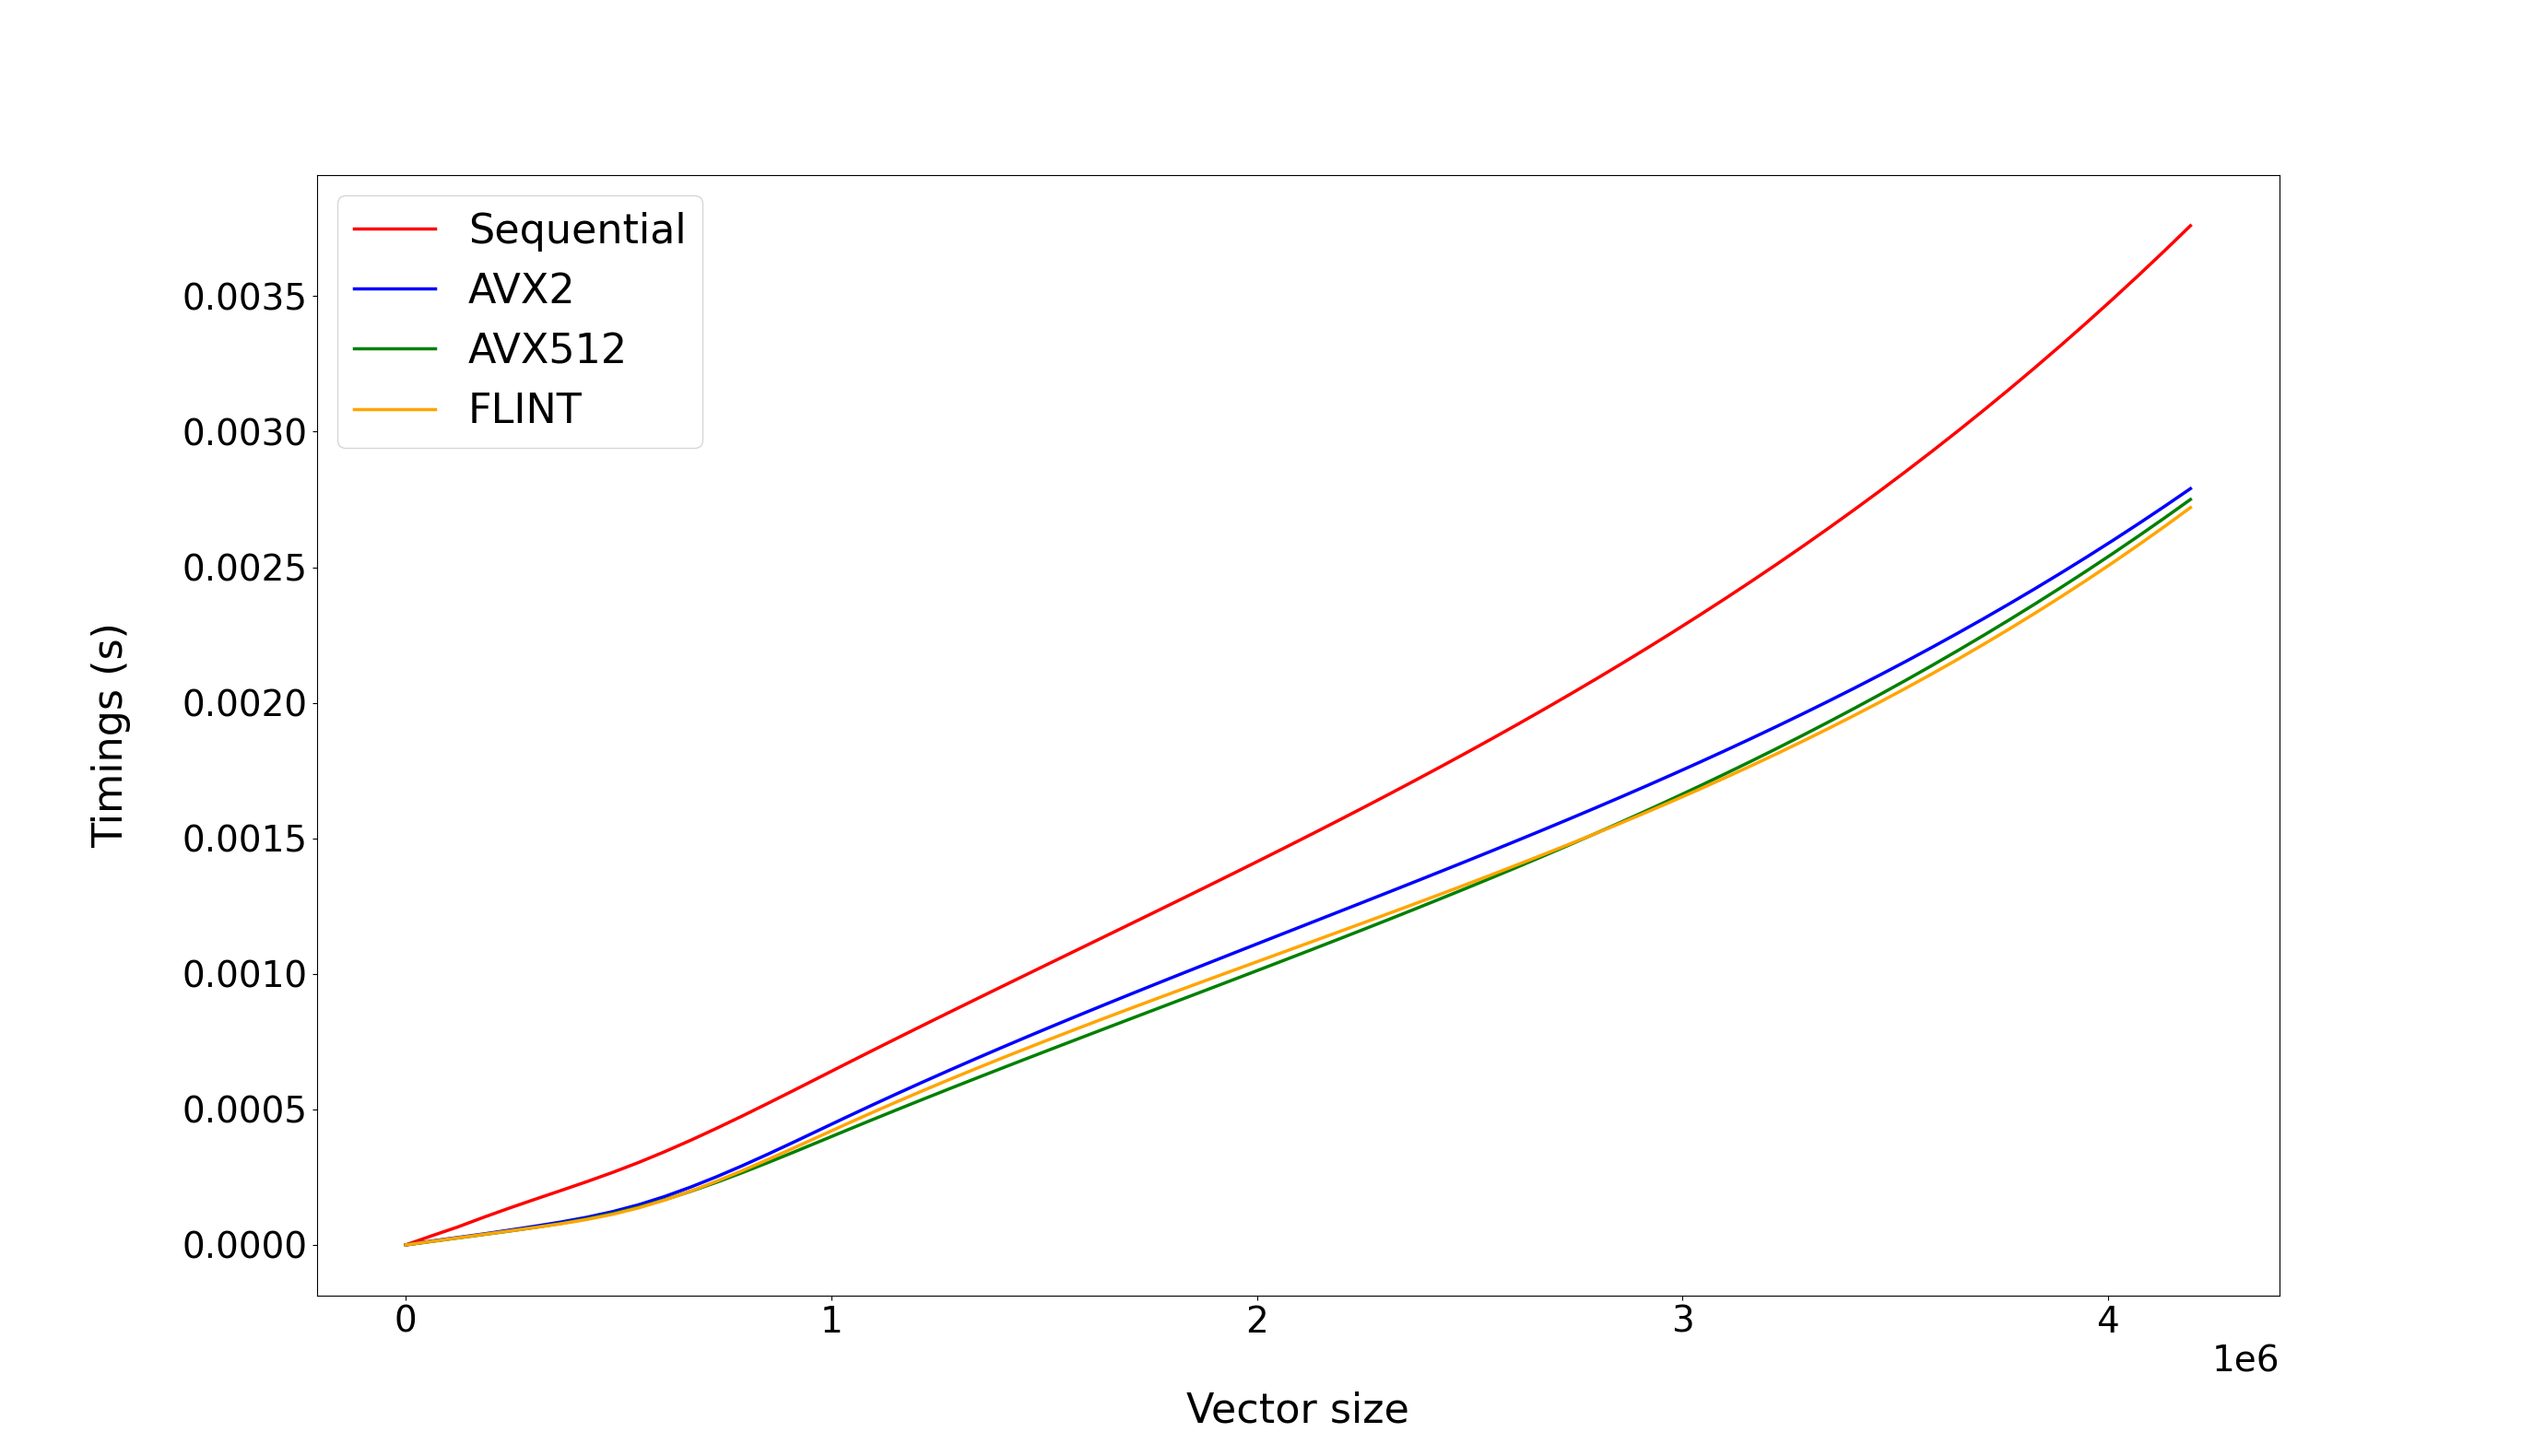
\includegraphics[width=1\textwidth]{add-mod_argiope.png}
        \end{center}
        %\caption{Timings in seconds of the modular sum with a 60-bit modulus on a Zen 4 processor.}
    \end{figure}
\end{frame}

\subsection{Multiplication of a vector by a scalar}
\begin{frame}
    \frametitle{Scalar vector product with a 60-bit modulus (1)}

    \begin{table}[h!]
        \centering
        
        % Proc 1: ppti
        \begin{tabular}{|r|*{3}{c c|}}
            \hline
            \rowcolor{myGray} 
            \multicolumn{7}{|c|}{\textsc{Cascade Lake}} \\
    
            \hline
            \rowcolor{myGray}
            Ver.\textbackslash N & 510 & & 2010 & & 32768 & \\
            \hline
            \cellcolor{myGray} Seq. & 5.92e-07 & 1.0x & 2.25e-06 & 1.0x & 5.58e-05 & 1.0x \\
            \hline
            \cellcolor{myGray} AVX2 & 7.26e-07 & 0.8x & 2.78e-06 & 0.8x & 4.88e-05 & 0.9x \\
            \hline
            \cellcolor{myGray} AVX512 & 3.52e-07 & 1.7x & 1.23e-06 & 1.8x & 2.36e-05 & 1.4x \\
            \hline
            \cellcolor{myGray} FLINT & 7.38e-07 & 1.0x & 2.82e-06 & 1.0x & 4.77e-05 & 0.9x \\
            \hline
        \end{tabular}
    
        % Proc 2: groebner
        \begin{tabular}{|r|*{3}{c c|}}
            \hline
            \rowcolor{myGray} 
            \multicolumn{7}{|c|}{\textsc{Ice Lake}} \\
    
            \hline
            \rowcolor{myGray}
            Ver.\textbackslash N & 510 & & 2010 & & 32768 & \\
            \hline
            \cellcolor{myGray} Seq. & 4.96e-07 & 1.0x & 1.92e-06 & 1.0x & 3.58e-05 & 1.0x \\
            \hline
            \cellcolor{myGray} AVX2 & 4.38e-07 & 1.1x & 1.70e-06 & 1.1x & 3.27e-05 & 0.9x \\
            \hline
            \cellcolor{myGray} AVX512 & 1.96e-07 & 2.5x & 7.44e-07 & 2.5x & 1.55e-05 & 2.1x \\
            \hline
            \cellcolor{myGray} FLINT & 4.50e-07 & 1.0x & 1.76e-06 & 1.0x & 3.36e-05 & 0.9x \\
            \hline
        \end{tabular}
    
        % Proc 3: argiope
        \begin{tabular}{|r|*{3}{c c|}}
            \hline
            \rowcolor{myGray}
            \multicolumn{7}{|c|}{\textsc{Zen 4}} \\
    
            \hline
            \rowcolor{myGray}
            Ver.\textbackslash N & 510 & & 2010 & & 32768 & \\
            \hline
            \cellcolor{myGray} Seq. & 3.35e-07 & 1.0x & 1.29e-06 & 1.0x & 2.17e-05 & 1.0x \\
            \hline
            \cellcolor{myGray} AVX2 & 2.35e-07 & 1.4x & 9.19e-07 & 1.4x & 1.56e-05 & 1.3x \\
            \hline
            \cellcolor{myGray} AVX512 & 1.16e-07 & 2.9x & 4.55e-07 & 2.8x & 7.53e-06 & 2.8x \\
            \hline
            \cellcolor{myGray} FLINT & 2.40e-07 & 1.0x & 9.29e-07 & 1.0x & 1.59e-05 & 1.0x \\
            \hline
        \end{tabular}
        %\caption{Timings in seconds and ratios of the modular scalar vector product with a 60-bit modulus.}
    \end{table}
\end{frame}

\begin{frame}
    \frametitle{Scalar vector product with a 60-bit modulus (2)}

    \begin{figure}[h!]
        \begin{center}
            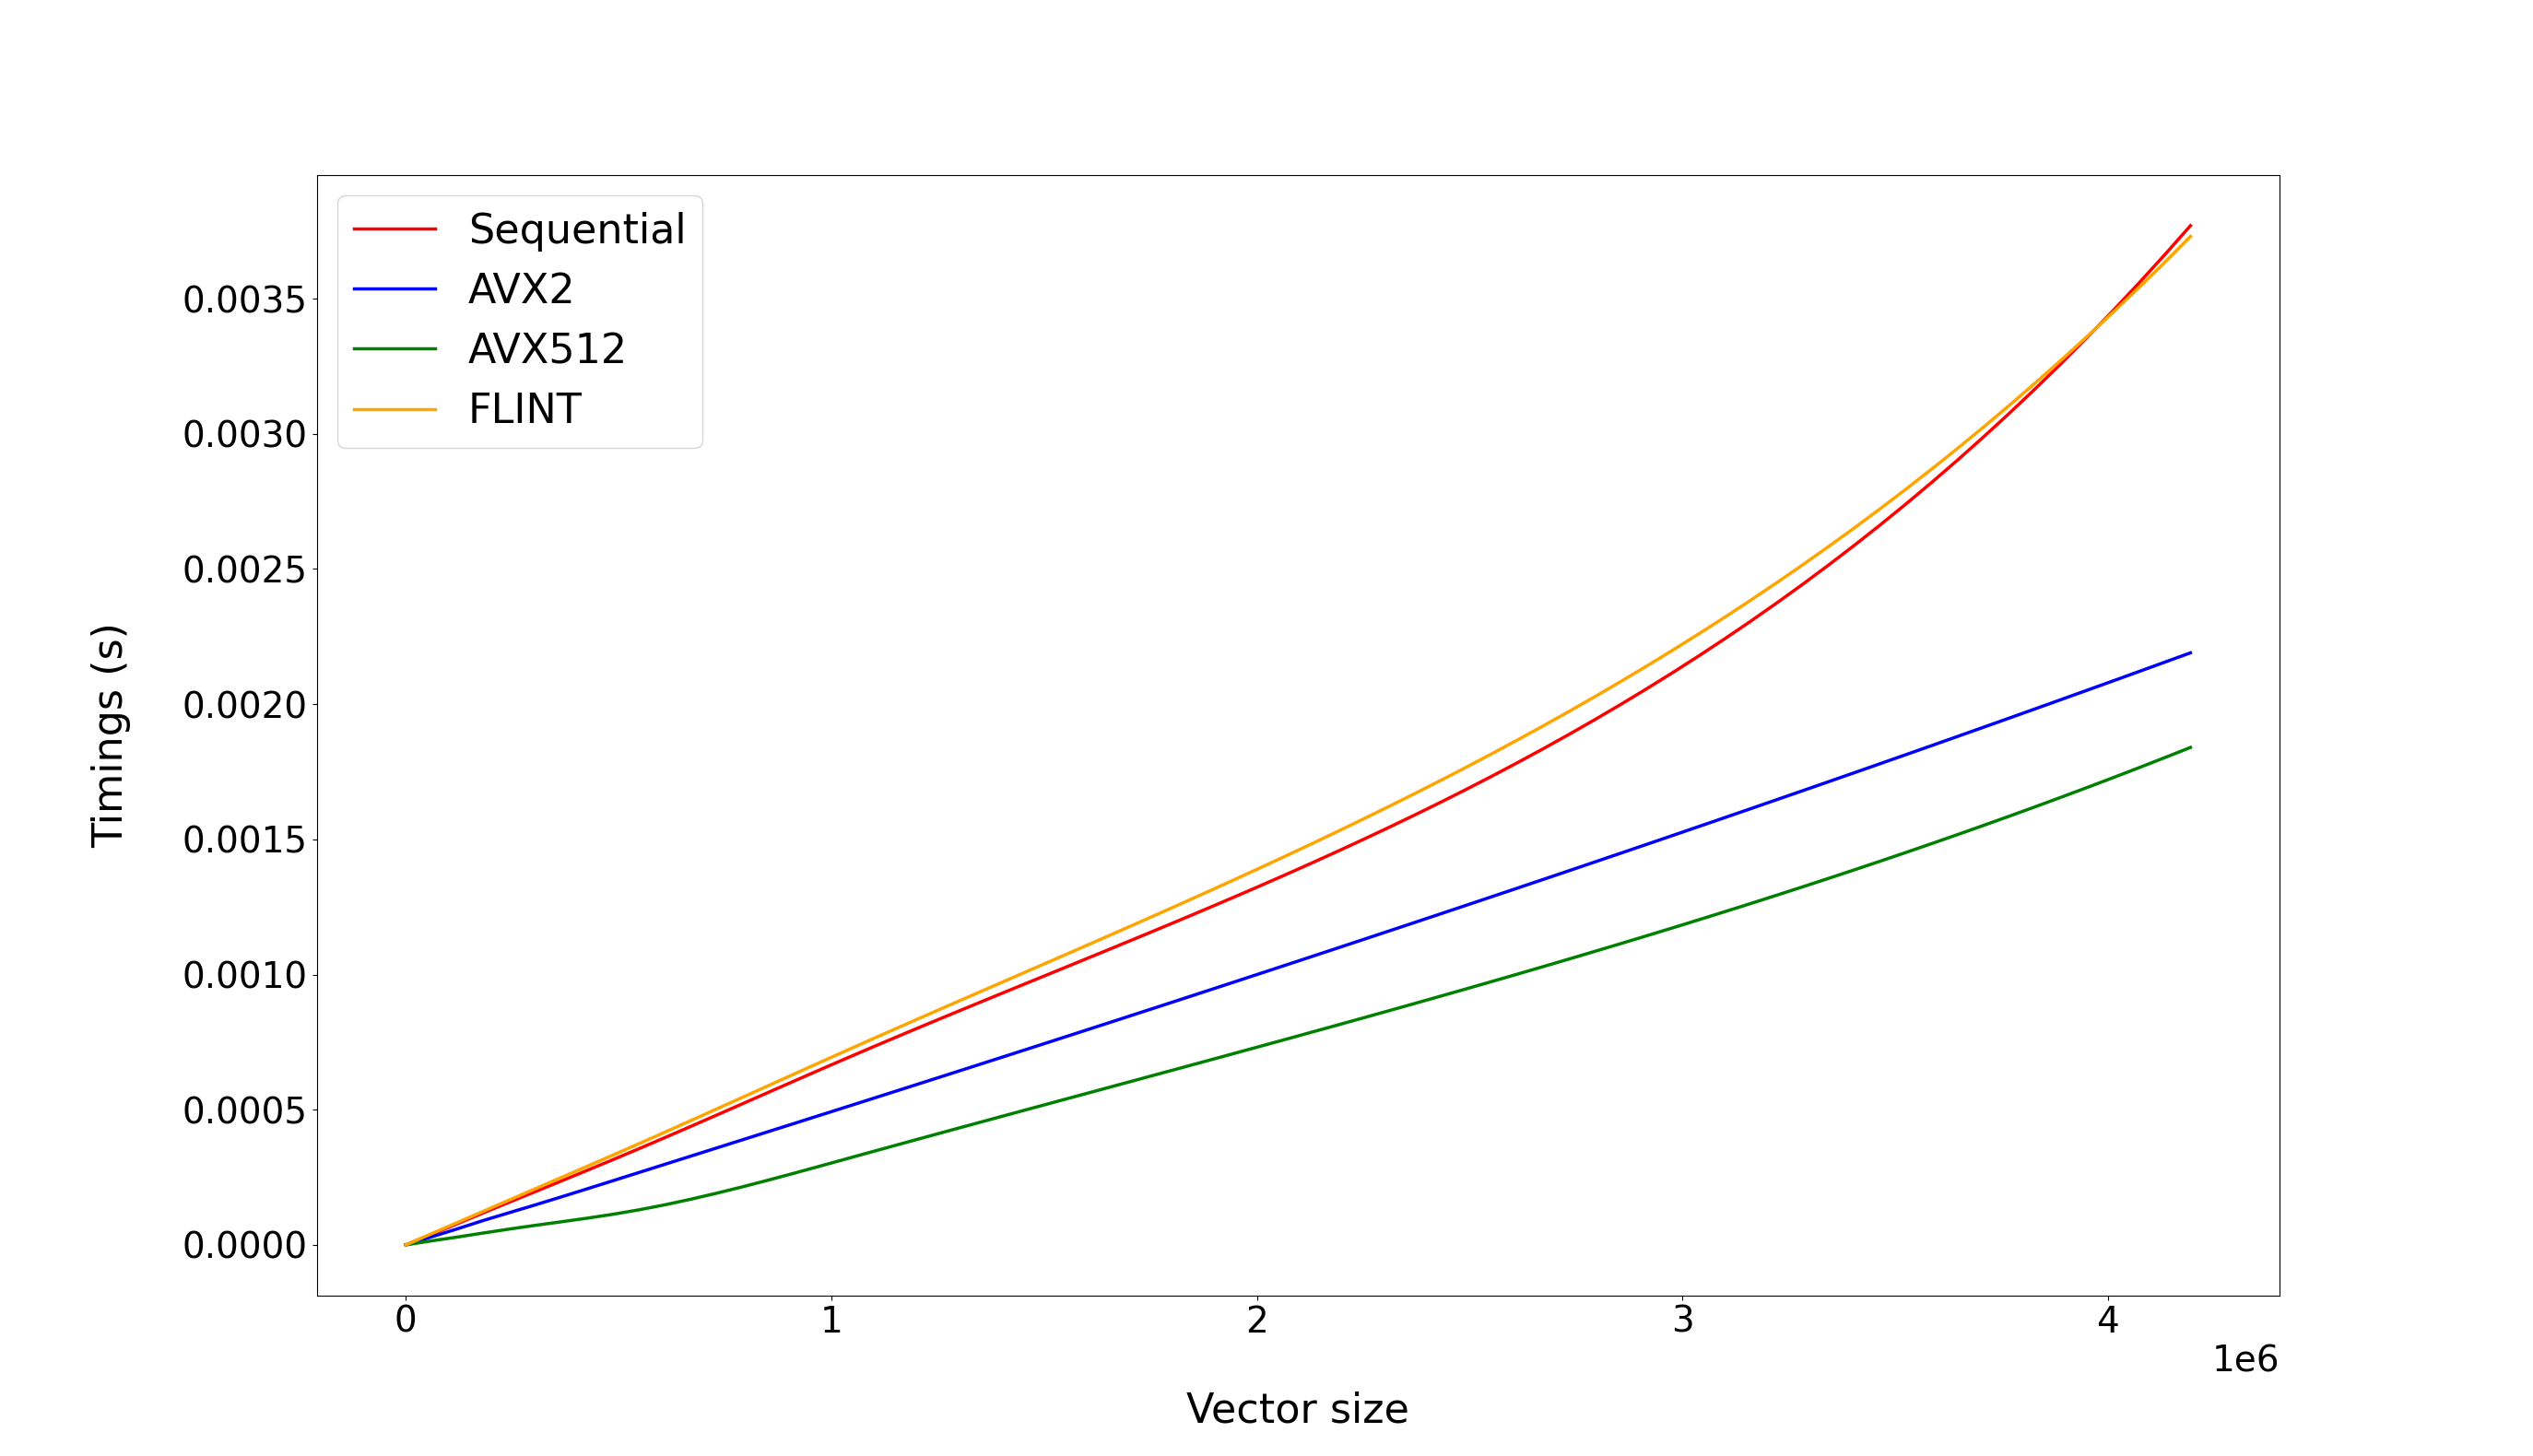
\includegraphics[width=1\textwidth]{scalar-vector-mod_argiope.png}
        \end{center}
        %\caption{Timings in seconds of the modular scalar vector product with a 60-bit modulus on a Zen 4 processor.}
    \end{figure}
\end{frame}

\subsection{Dot product}
\begin{frame}
    \frametitle{Dot product}
    Given two vector $a = (a_1,\cdots,a_N), b = (b_1,\cdots b_N) \in \left(\mathbb{Z}/n\mathbb{Z}\right)^N$
    \[
        \left(\sum^N_{i=1}a_i\cdot b_i\right) \mod n
    \]
    %with $n$ of size $k$ bits

    \medskip
    \begin{itemize}
        \item<+-> Modular reduction performed at the end of the sum
            \begin{itemize}
                \item[$+$] Improve performance
                \item[$-$] Limit the vectors size to avoid overflow
            \end{itemize}
        \item<+-> When using long multiplication
            \begin{enumerate}
                \item Compute separate sums for the three limbs ($r_{hi}$, $r_{mi}$, $r_{lo}$)
                \item Reconstruct the result
            \end{enumerate}
    \end{itemize}
\end{frame}

\begin{frame}
    \frametitle{Dot product with a 60-bit modulus (1)}

    \begin{table}[h!]
        \centering
        
        % Proc 1: ppti
        \begin{tabular}{|r|*{3}{c c|}}
            \hline
            \rowcolor{myGray} 
            \multicolumn{7}{|c|}{\textsc{Cascade Lake}} \\
    
            \hline
            \rowcolor{myGray}
            Ver.\textbackslash N & 510 & & 2010 & & 32768 & \\
            \hline
            \cellcolor{myGray} Seq. & 2.84e-07 & 1.0x & 1.11e-06 & 1.0x & 1.92e-05 & 1.0x \\
            \hline
            \cellcolor{myGray} AVX2 & 2.97e-07 & 1.0x & 1.12e-06 & 1.0x & 1.94e-05 & 1.0x \\
            \hline
            \cellcolor{myGray} AVX512 & 2.16e-07 & 1.3x & 7.74e-07 & 1.4x & 1.44e-05 & 1.3x \\
            \hline
            \cellcolor{myGray} FLINT & 3.18e-07 & 0.9x & 1.18e-06 & 0.9x & 1.98e-05 & 1.0x \\
            \hline
        \end{tabular}
    
        % Proc 2: groebner
        \begin{tabular}{|r|*{3}{c c|}}
            \hline
            \rowcolor{myGray} 
            \multicolumn{7}{|c|}{\textsc{Ice Lake}} \\
    
            \hline
            \rowcolor{myGray}
            Ver.\textbackslash N & 510 & & 2010 & & 32768 & \\
            \hline
            \cellcolor{myGray} Seq. & 4.20e-07 & 1.0x & 1.54e-06 & 1.0x & 2.50e-05 & 1.0x \\
            \hline
            \cellcolor{myGray} AVX2 & 1.72e-07 & 2.3x & 6.45e-07 & 2.4x & 1.20e-05 & 2.1x \\
            \hline
            \cellcolor{myGray} AVX512 & 1.67e-07 & 2.4x & 6.13e-07 & 2.5x & 1.30e-05 & 1.9x \\
            \hline
            \cellcolor{myGray} FLINT & 2.87e-07 & 1.4x & 9.58e-07 & 1.6x & 1.77e-05 & 1.4x \\
            \hline
        \end{tabular}
    
        % Proc 3: argiope
        \begin{tabular}{|r|*{3}{c c|}}
            \hline
            \rowcolor{myGray}
            \multicolumn{7}{|c|}{\textsc{Zen 4}} \\
    
            \hline
            \rowcolor{myGray}
            Ver.\textbackslash N & 510 & & 2010 & & 32768 & \\
            \hline
            \cellcolor{myGray} Seq. & 2.70e-07 & 1.0x & 1.20e-06 & 1.0x & 1.68e-05 & 1.0x \\
            \hline
            \cellcolor{myGray} AVX2 & 1.20e-07 & 2.6x & 3.87e-07 & 2.6x & 5.85e-06 & 2.9x \\
            \hline
            \cellcolor{myGray} AVX512 & 1.10e-07 & 2.7x & 3.78e-07 & 2.7x & 5.46e-06 & 3.1x \\
            \hline
            \cellcolor{myGray} FLINT & 2.70e-07 & 1.3x & 8.48e-07 & 1.2x & 1.34e-05 & 1.3x \\
            \hline
        \end{tabular}
        %\caption{Timings in seconds and ratios of the modular dot product with a 60-bit modulus.}
    \end{table}
\end{frame}
    
\begin{frame}
    \frametitle{Dot product with a 60-bit modulus (2)}

    \begin{figure}[h!]
        \begin{center}
            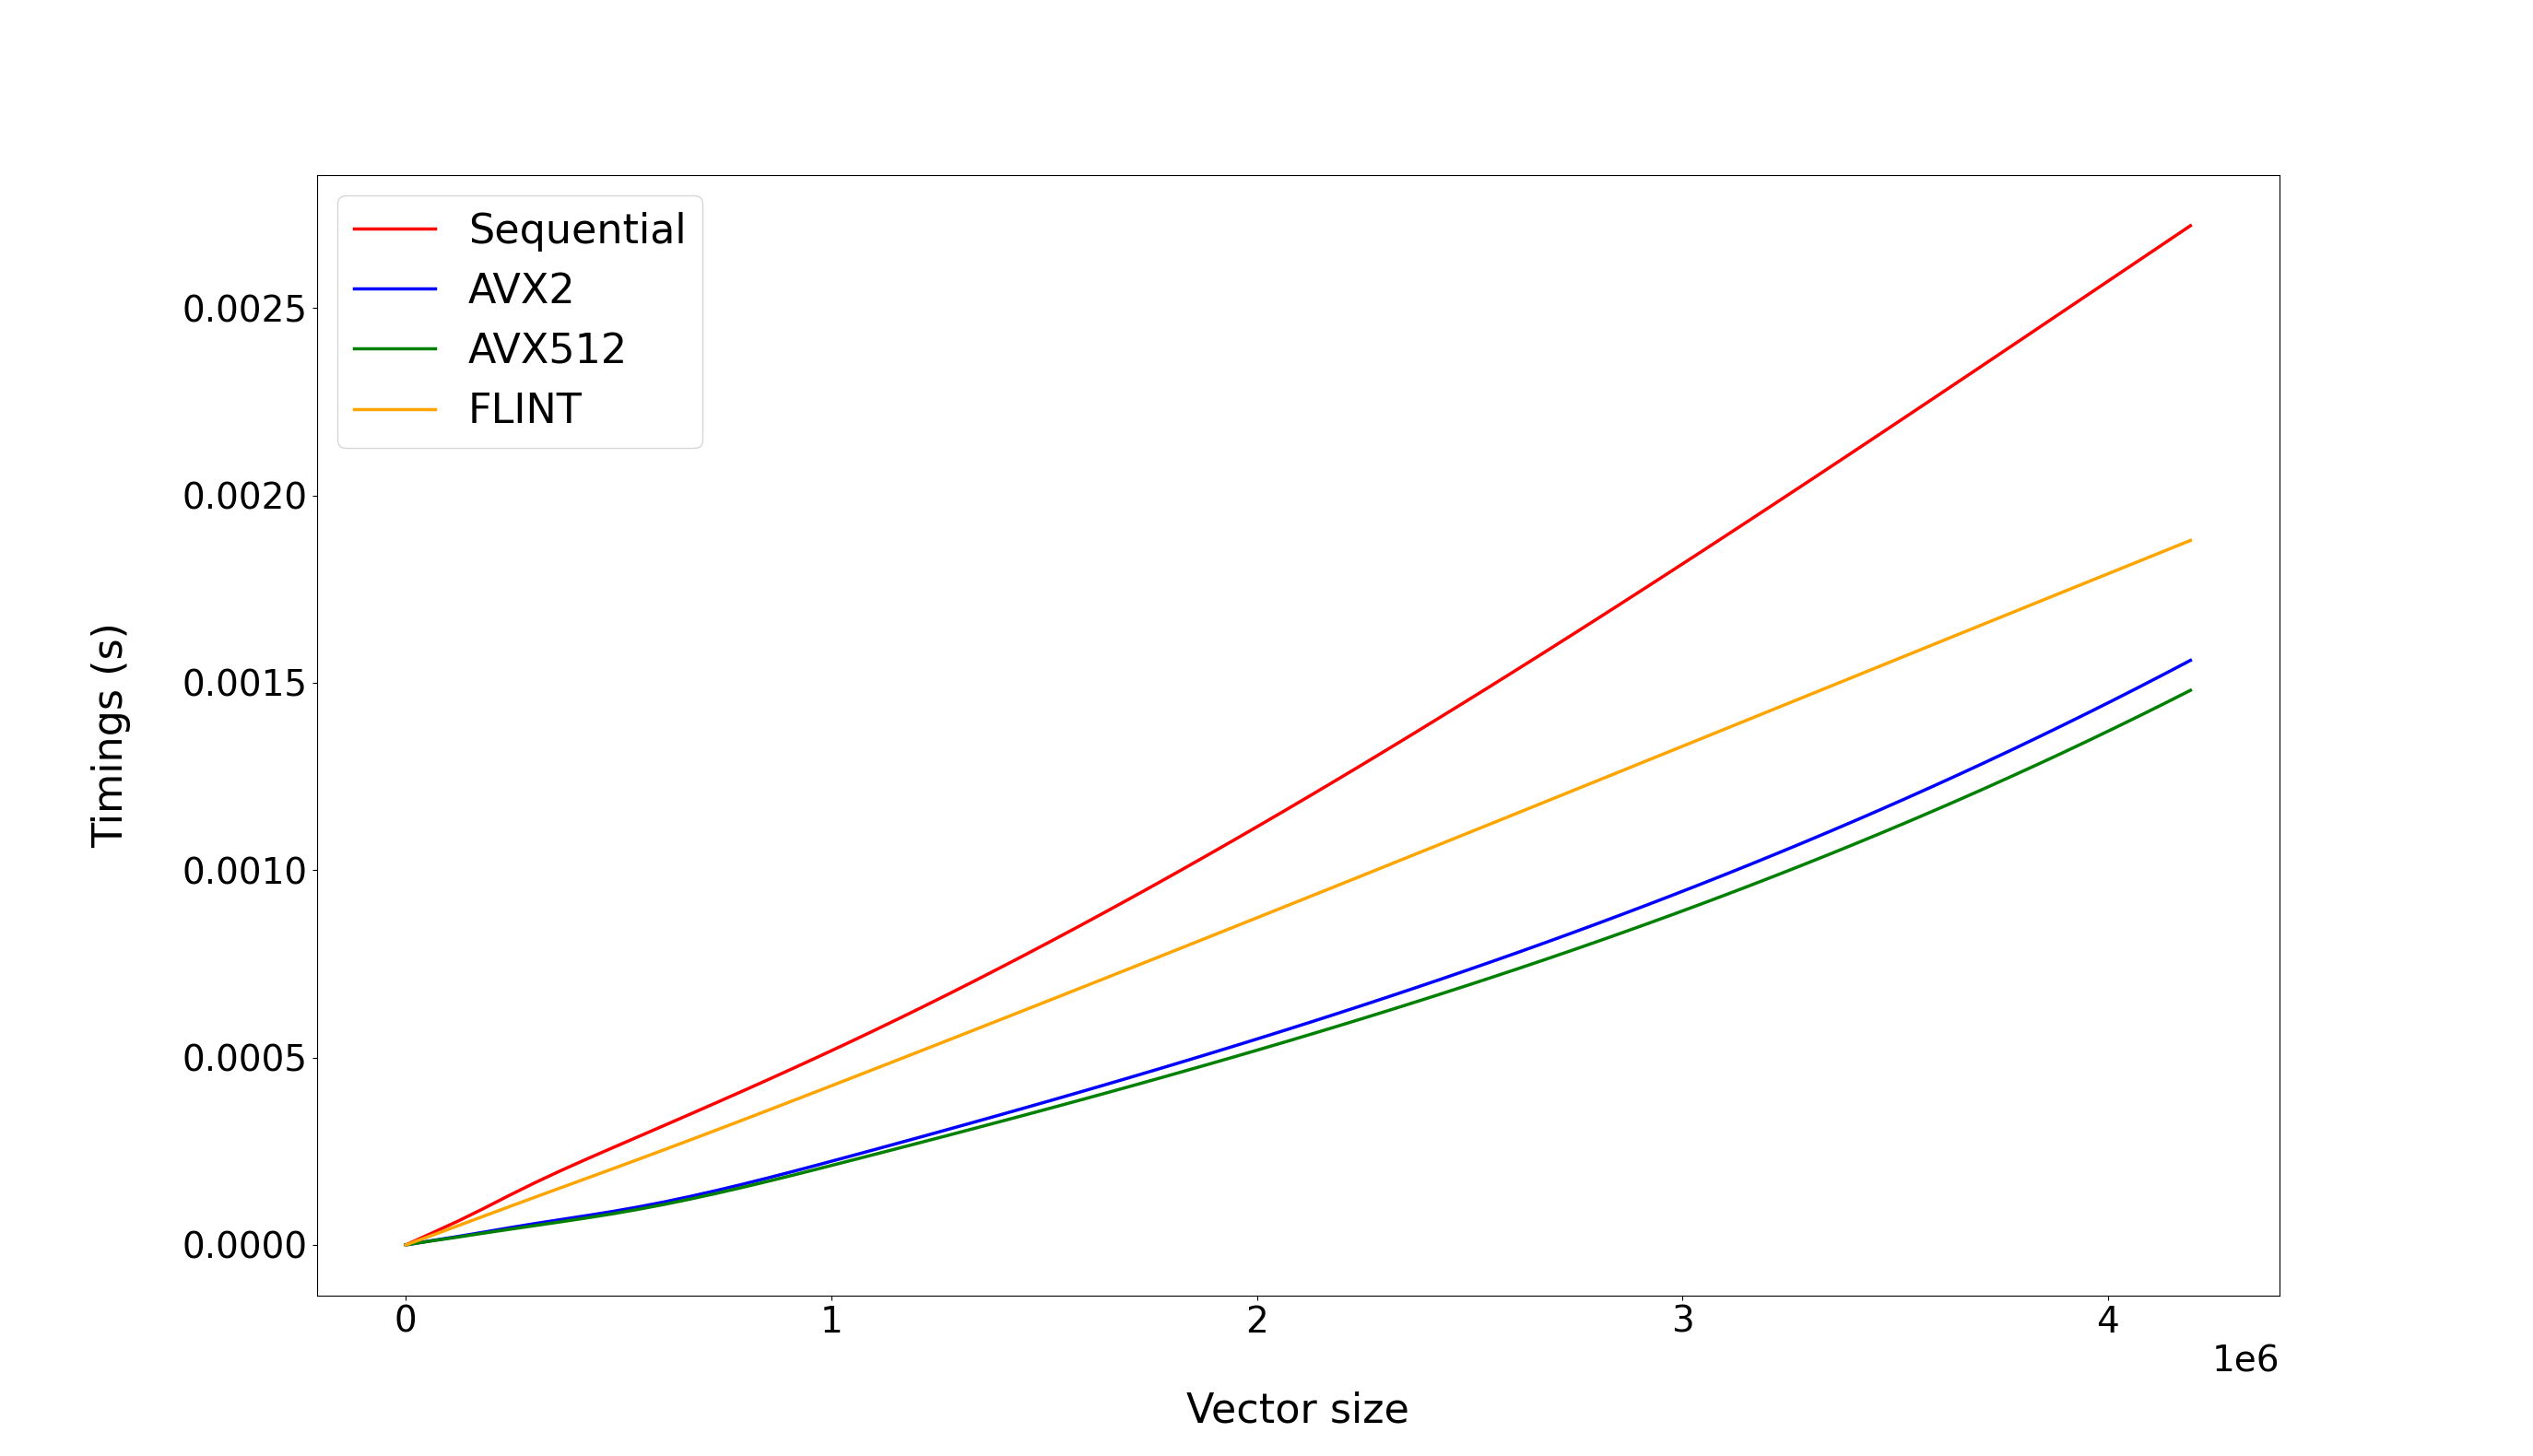
\includegraphics[width=1\textwidth]{dot-prod-mod_argiope.png}
        \end{center}
        %\caption{Timings in seconds of the modular dot product with a 60-bit modulus on a Zen 4 processor.}
    \end{figure}
\end{frame}

\section{Butterfly Fast Fourier Transform}
\subsection{Harvey lazy butterfly FFT}
\begin{frame}
    \frametitle{Butterfly Fast Fourier Transform}
    \begin{mybox}
    Let $w, n$ be integers, $x,y \in \mathbb{Z}/n\mathbb{Z}$, 
    the \textit{butterfly FFT} is the in-place transformation: 
    \[
    (x,y) \mapsto (x + w\cdot y \mod n,\ x - w\cdot y \mod n).
    \]
    \end{mybox}
    
    \pause
    \bigskip
    \textbf{Harvey lazy butterfly algorithm\cite{DBLP:journals/corr/abs-1205-2926}:}

    \medskip
    For $n < \textcolor{red}{2^B /4}$, $x,y < \textcolor{red}{4n}$, $(w, w_{pre})$,
    \begin{enumerate}
        \item $x \gets \min(x-2n, x)$,
        \item compute $p_{hi}, p_{lo}$ such that $w_{pre} \cdot b_i = p_{hi}\cdot 2^B + p_{lo}$, \hfill (1 \code{mulhi})
        \item $c \gets w\cdot b_i - p_{hi}\cdot n$, \hfill (2 \code{mullo})
        \item $c \gets \min(c-2n, c)$,
        \item $x\gets x + c$ \\
            $y \gets x - c + 2n$
        \item return $x,y$
    \end{enumerate}

\end{frame}

\begin{frame}
    \frametitle{Lazy butterfly FFT with a 60-bit modulus (1)}

    \begin{table}[h!]
        \centering
        
        % Proc 1: ppti
        \begin{tabular}{|r|*{3}{c c|}}
            \hline
            \rowcolor{myGray} 
            \multicolumn{7}{|c|}{\textsc{Cascade Lake}} \\
    
            \hline
            \rowcolor{myGray}
            Ver.\textbackslash N & 510 & & 2010 & & 32768 & \\
            \hline
            \cellcolor{myGray} Seq. & 8.13e-07 & 1.0x & 3.18e-06 & 1.0x & 5.28e-05 & 1.0x \\
            \hline
            \cellcolor{myGray} AVX2 & 7.46e-07 & 1.1x & 2.88e-06 & 1.1x & 4.71e-05 & 1.1x \\
            \hline
            \cellcolor{myGray} AVX512 & 3.87e-07 & 2.1x & 1.56e-06 & 2.0x & 3.17e-05 & 1.7x \\
            \hline
        \end{tabular}
    
        % Proc 2: groebner
        \begin{tabular}{|r|*{3}{c c|}}
            \hline
            \rowcolor{myGray} 
            \multicolumn{7}{|c|}{\textsc{Ice Lake}} \\
    
            \hline
            \rowcolor{myGray}
            Ver.\textbackslash N & 510 & & 2010 & & 32768 & \\
            \hline
            \cellcolor{myGray} Seq. & 7.37e-07 & 1.0x & 2.92e-06 & 1.0x & 4.77e-05 & 1.0x \\
            \hline
            \cellcolor{myGray} AVX2 & 5.25e-07 & 1.4x & 2.40e-06 & 1.4x & 3.38e-05 & 1.4x \\
            \hline
            \cellcolor{myGray} AVX512 & 2.24e-07 & 3.3x & 9.37e-07 & 3.1x & 1.69e-05 & 2.8x \\
            \hline
        \end{tabular}
    
        % Proc 3: argiope
        \begin{tabular}{|r|*{3}{c c|}}
            \hline
            \rowcolor{myGray}
            \multicolumn{7}{|c|}{\textsc{Zen 4}} \\
    
            \hline
            \rowcolor{myGray}
            Ver.\textbackslash N & 510 & & 2010 & & 32768 & \\
            \hline
            \cellcolor{myGray} Seq. & 5.30e-07 & 1.0x & 2.30e-06 & 1.0x & 3.39e-05 & 1.0x \\
            \hline
            \cellcolor{myGray} AVX2 & 2.87e-07 & 1.8x & 1.12e-06 & 1.8x & 1.79e-05 & 1.9x \\
            \hline
            \cellcolor{myGray} AVX512 & 1.44e-07 & 3.5x & 5.80e-07 & 3.5x & 9.12e-06 & 3.7x \\
            \hline
        \end{tabular}
        %\caption{Timings in seconds and ratios of the Harvey lazy butterfly FFT with a 60-bit modulus.}
    \end{table}
\end{frame}

\begin{frame}
    \frametitle{Lazy butterfly FFT with a 60-bit modulus (2)}

    \begin{figure}[h!]
        \begin{center}
            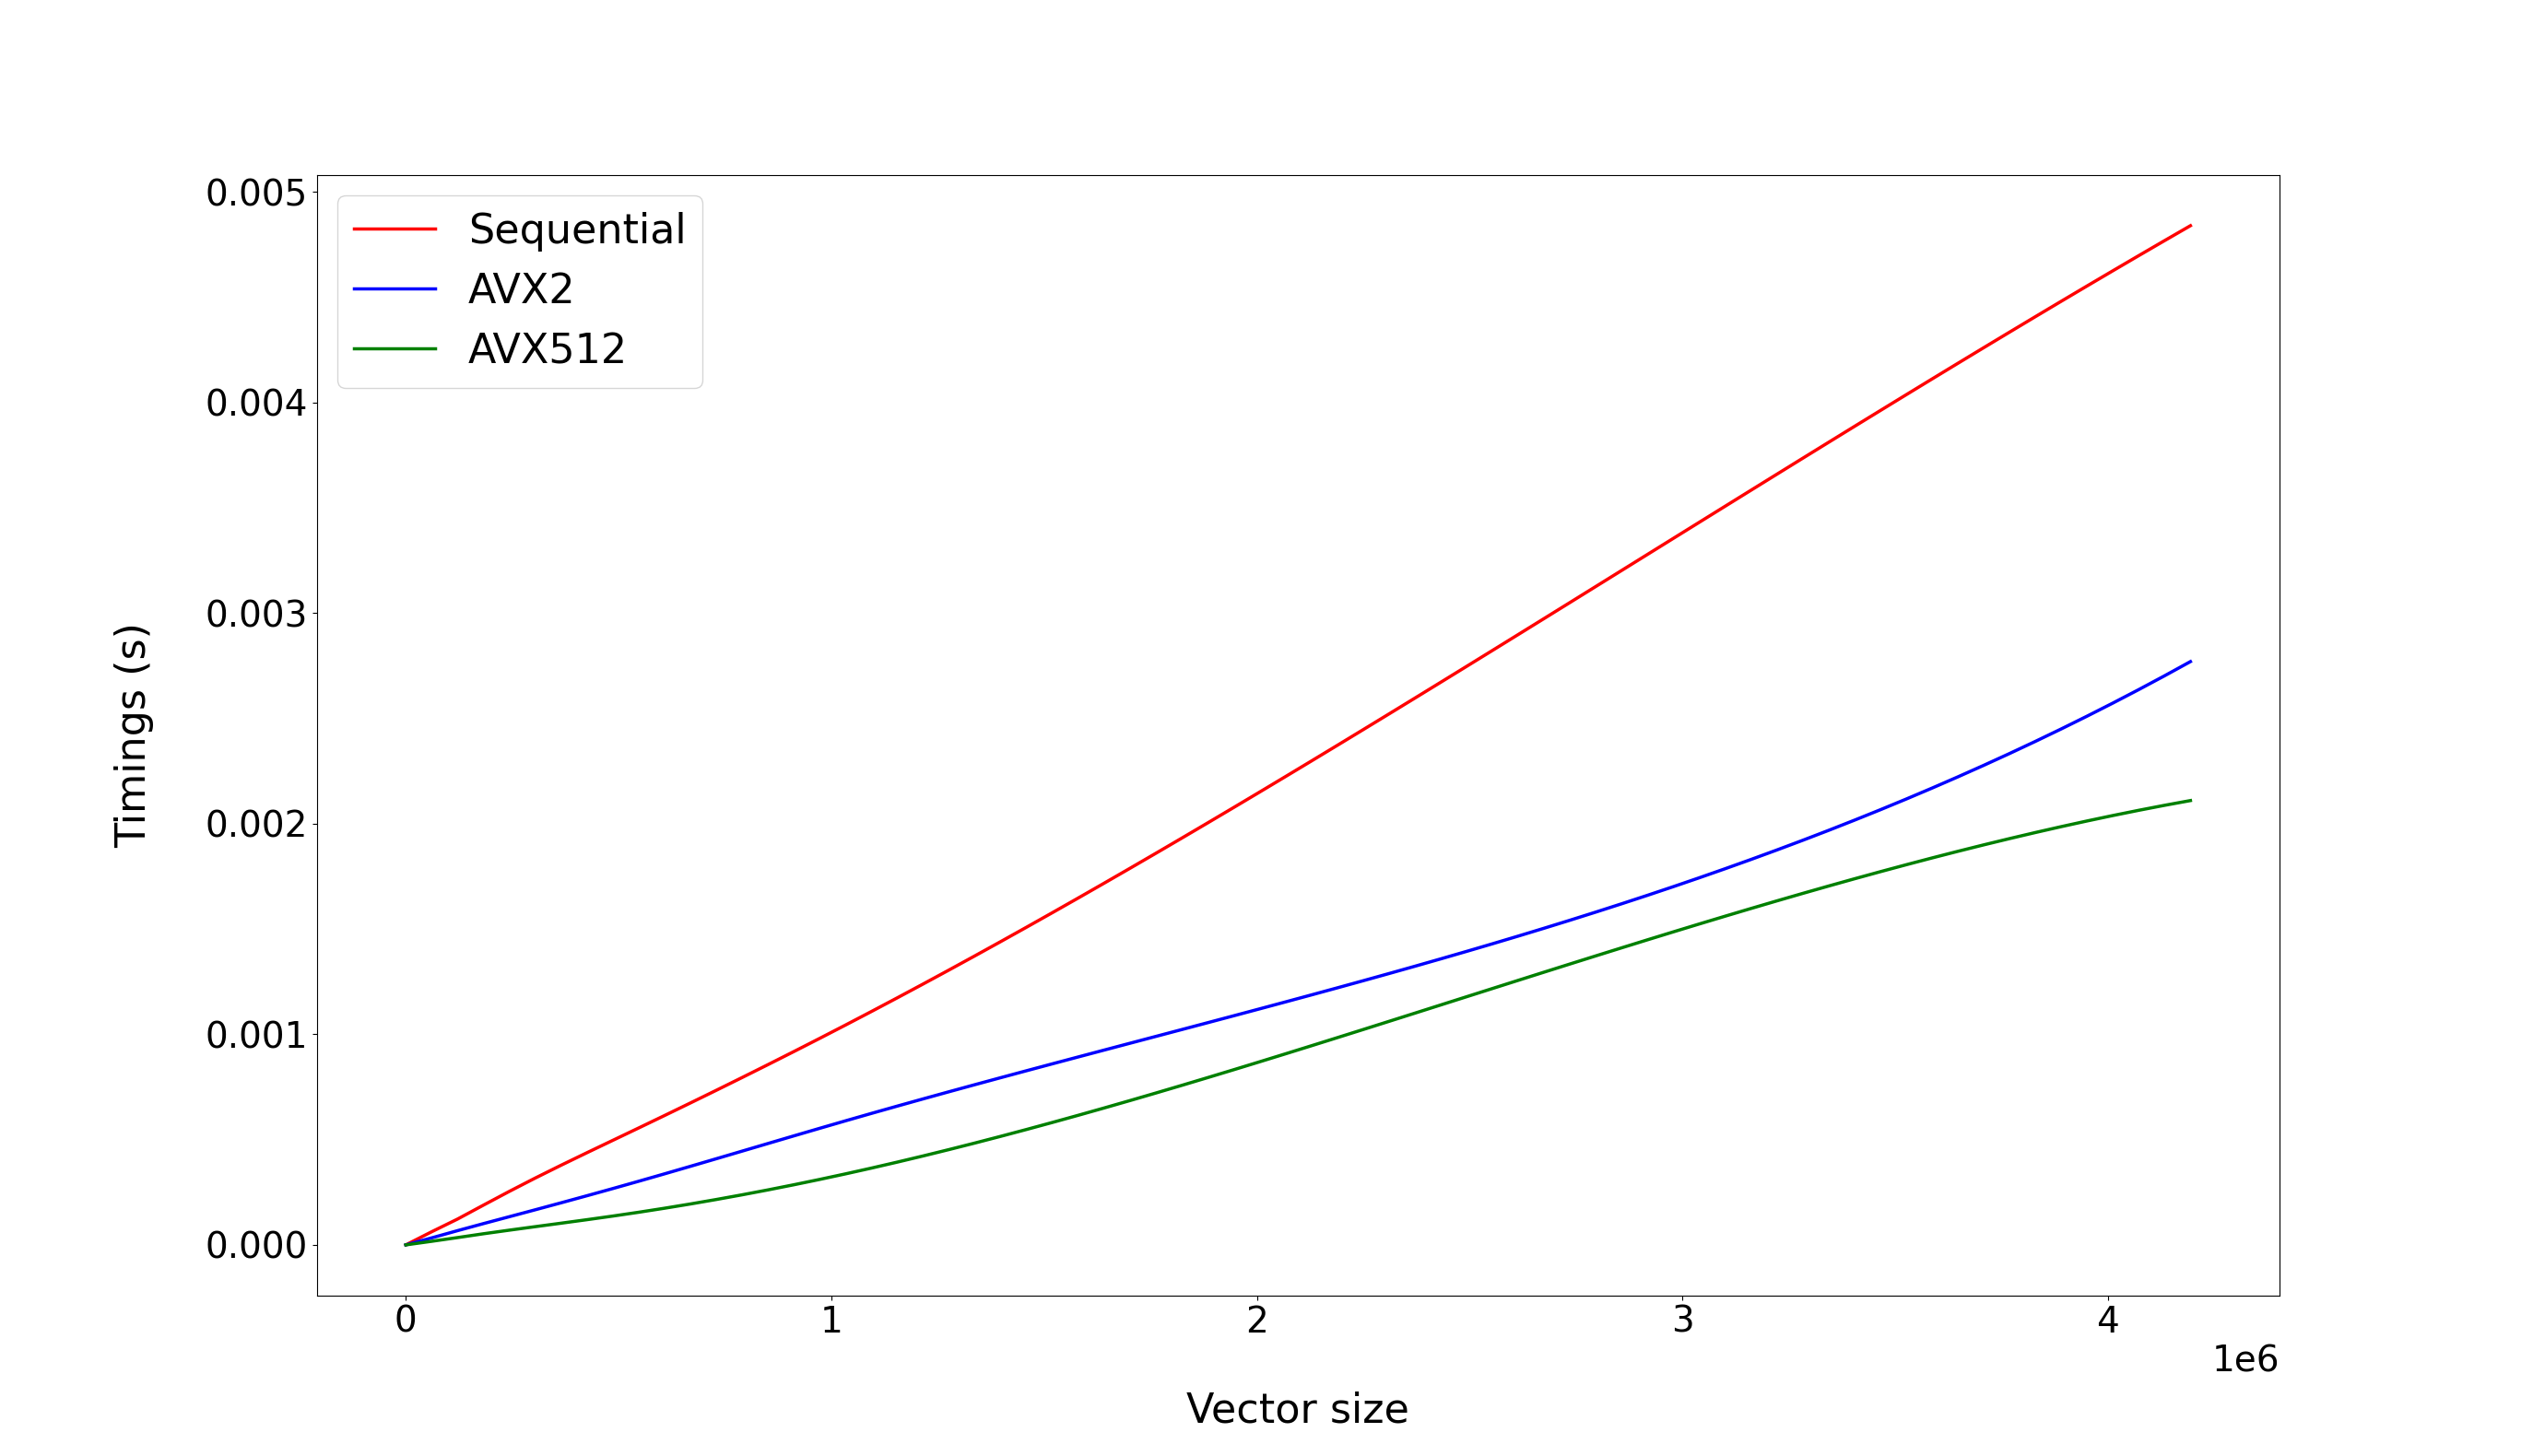
\includegraphics[width=1\textwidth]{lazy-butterfly_argiope.png}
        \end{center}
        %\caption{Timings in seconds of the Harvey lazy butterfly FFT with a 60-bit modulus on a Zen 4 processor.}
    \end{figure}
\end{frame}

\subsection{Consequences on a complete FFT implementation}
\begin{frame}
    \frametitle{FFT with a 50-bit prime modulus}

    \begin{center}
        \scalebox{0.75}{
        \begin{tabular}{|r|*{4}{c|}}
            \hline
            \rowcolor{myGray}
            depth & sd\_fft & dft4 & dft4s & dft2s \\
            \hline
            \cellcolor{myGray} 3 & 1.5e-08 & 1.4e-08 & 1.5e-08 & 1.5e-08 \\
            \hline
            \cellcolor{myGray} 4 & 2.1e-08 & 3.5e-08 & 2.2e-08 & 2.4e-08 \\
            \hline
            \cellcolor{myGray} 5 & 2.7e-08 & 8.2e-08 & 5.4e-08 & 5.3e-08 \\
            \hline
            \cellcolor{myGray} 6 & 6.2e-08 & 2.0e-07 & 9.7e-08 & 1.1e-07 \\
            \hline
            \cellcolor{myGray} 7 & 1.1e-07 & 4.4e-07 & 2.3e-07 & 2.3e-07 \\
            \hline
            \cellcolor{myGray} 8 & 2.9e-07 & 1.1e-06 & 4.8e-07 & 5.2e-07 \\
            \hline
            \cellcolor{myGray} 9 & 5.6e-07 & 2.3e-06 & 1.1e-06 & 1.1e-06 \\
            \hline
            \cellcolor{myGray} 10 & 1.3e-06 & 5.4e-06 & 2.2e-06 & 2.5e-06 \\
            \hline
            \cellcolor{myGray} 11 & 2.9e-06 & 1.1e-05 & 5.0e-06 & 5.0e-06 \\
            \hline
            \cellcolor{myGray} 12 & 6.1e-06 & 2.5e-05 & 1.0e-05 & 1.1e-05 \\
            \hline
            \cellcolor{myGray} 13 & 1.3e-05 & 5.3e-05 & 2.4e-05 & 2.4e-05 \\
            \hline
            \cellcolor{myGray} 14 & 2.9e-05 & 1.2e-04 & 4.8e-05 & 5.0e-05 \\
            \hline
            \cellcolor{myGray} 15 & 6.1e-05 & 2.4e-04 & 1.0e-04 & 1.1e-04 \\
            \hline
            \cellcolor{myGray} 16 & 1.3e-04 & 5.2e-04 & 2.0e-04 & 2.2e-04 \\
            \hline
            \cellcolor{myGray} 17 & 2.7e-04 & 1.1e-03 & 4.5e-04 & 4.6e-04 \\
            \hline
            \cellcolor{myGray} 18 & 5.8e-04 & 2.4e-03 & 9.1e-04 & 9.6e-04 \\
            \hline
            \cellcolor{myGray} 19 & 1.2e-03 & 4.9e-03 & 2.0e-03 & 2.0e-03 \\
            \hline
            \cellcolor{myGray} 20 & 2.6e-03 & 1.1e-02 & 4.1e-03 & 4.3e-03 \\
            \hline
            \cellcolor{myGray} 21 & 6.0e-03 & 2.2e-02 & 9.2e-03 & 9.6e-03 \\
            \hline
            \cellcolor{myGray} 22 & 1.3e-02 & 4.8e-02 & 2.0e-02 & 2.3e-02 \\
            \hline
            \cellcolor{myGray} 23 & 2.8e-02 & 9.9e-02 & 4.2e-02 & 4.7e-02 \\
            \hline
            \cellcolor{myGray} 24 & 6.2e-02 & 2.1e-01 & 8.3e-02 & 9.8e-02 \\
            \hline
            \cellcolor{myGray} 25 & 1.3e-01 & 4.4e-01 & 1.8e-01 & 2.1e-01 \\
            \hline
        \end{tabular}
        }
    \end{center}
\end{frame}

\section{Conclusion}
\begin{frame}
    \frametitle{Open questions}

    \textbf{Special primes}
    \begin{itemize}
        \item Mersenne numbers: $n\in \mathbb{N}$,
            $$M_n = 2^n - 1.$$
        \item Generalized Mersenne primes of the form:
            \begin{align*}
                p &= 2^u + 2^v + 1 \\ 
                p &= 2^u - 2^v + 1 
            \end{align*}
            of $u+1$ bits, with $64 > u > v > 0$.
    \end{itemize}

    \bigskip
    \textbf{Integer Fused Multiply Add (IFMA) instructions}
    
    $\Longrightarrow$ Vectorization based on floating-point arithmetic.

\end{frame}

\section{References}
\begin{frame}
    \frametitle{References}

    \bibliographystyle{plain} 
    \bibliography{biblio} 
    \nocite{*}
\end{frame}

\end{document}
